\documentclass[a4paper, 12pt]{extarticle}
\usepackage[dvipsnames]{xcolor}
\usepackage[top=70pt,bottom=70pt,left=48pt,right=46pt]{geometry}
\definecolor{header}{RGB}{92,184,92}
\definecolor{defenition}{RGB}{217,83,79}
\definecolor{main_title}{RGB}{66,139,202}
\definecolor{sub_header}{RGB}{91,192,222}
\usepackage[english, russian]{babel}
\usepackage[utf8]{inputenc}
\usepackage{amsmath}
\usepackage{listings}
\usepackage{graphicx}
\usepackage{amsmath}
\title{\textcolor{main_title}{Определение петли гистерезиса магнитооптическим методом}}
\author{Шмаков Владимир Евгеньевич - ФФКЭ гр. Б04-105}






\begin{document}
\maketitle



\section*{\textcolor{header}{Цель работы}}
\begin{itemize}
    \item Ознакомление с принципами применения магнитооптических методов для исследования прозрачных магнетиков
    \item Определение магнитных параметров исследуемого образца 
\end{itemize}


\section*{\textcolor{header}{Теоретические сведения}}

Ферромагнетик в отсутствие внешнего поля может обладать значительной намагниченностью, вызванной упорядочиванием магнитных моментов из-за внутренних взаимодействий, главным образом обменного.
Возникающая магнитная структура представляет собой домены – области однородной намагниченности, разделённые доменными стенками. 
Основной причиной формирования доменов является стремление уменьшения вклада магнитостатической энергии, возникающего благодаря выходу нормальной составляющей намагниченности на поверхности образца. 
Форма магнитной структуры определяется уже более слабыми взаимодействиями, которые зависят от магнитостатической энергии структуры, кристаллографической анизотропии, энергии доменных границ, энергии взаимодействия с внешним магнитным полем.
В слабых полях рост намагниченности вызван ростом момента одних областей за счёт уменьшения других в результате сдвига границ. 
В сильных полях происходит поворот момента отдельных областей по полю, достигается насыщение. 
Если после получения основной кривой намагничивания постепенно убрать внешнее поле, то намагниченность вещества уже не ляжет на ту же кривую из-за произошедших необратимых изменений. 
Для обращения намагниченности образца в нуль необходимо приложить поле, называемое коэрцитивной силой. 
Это явление называется \textcolor{defenition}{магнитным гистерезисом}. 



\section*{\textcolor{header}{Методика}}
\subsection*{\textcolor{sub_header}{Оборудование}}
\begin{itemize}
    \item Лазер
    \item Образец 
    \item Катушка
    \item Поляроид
    \item Фотодиод
    \item Усилитель
    \item Амперметр
    \item Резистор 
    \item Осциллограф
    \item АЦП
\end{itemize}


\subsection*{\textcolor{sub_header}{Экспериментальная установка}}
\begin{figure}[htbp]
    \centering
    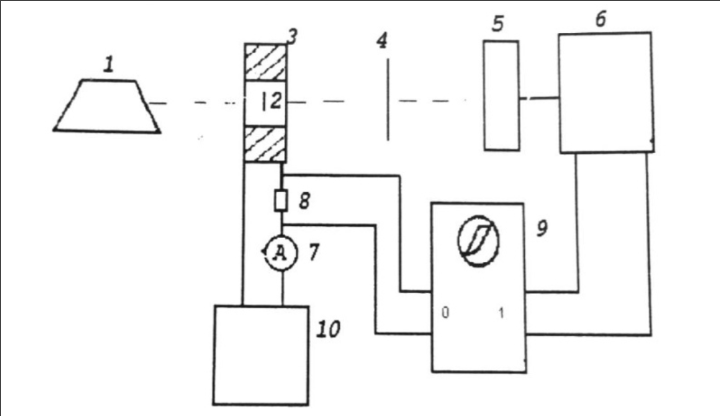
\includegraphics[width = 0.8 \textwidth]{setup.png}
    \caption{Блок-схема экспериментальной установки}
    \label{fig:setup}
\end{figure}

Для создания магнитного поля используются катушки(3). Линейно поляризованный
луч лазера(1) пропускается через образец. Вследствие магнитооптического эффекта,
поляризация луча искажается(угол поляризации изменяется). При этом искажение оказывается пропорционально величине
магнитного поля. Согласно закону Малюса, отклонение угла поляризации приводит к падению интенсивности света на фотодиоде.

На ось x осциллографа подаётся напряжение на резисторе 8. На ось y - сигнал с фотоприёмника. 
Таким образом, на экране наблюдается петля гистерезиса.


\section*{\textcolor{header}{Обработка экспериментальных данных}}

Экспериментальные данные представляют из себя два сигнала - напряжение на резисторе и напряжение на фотодиоде.
\begin{figure}[htbp]
    \centering
    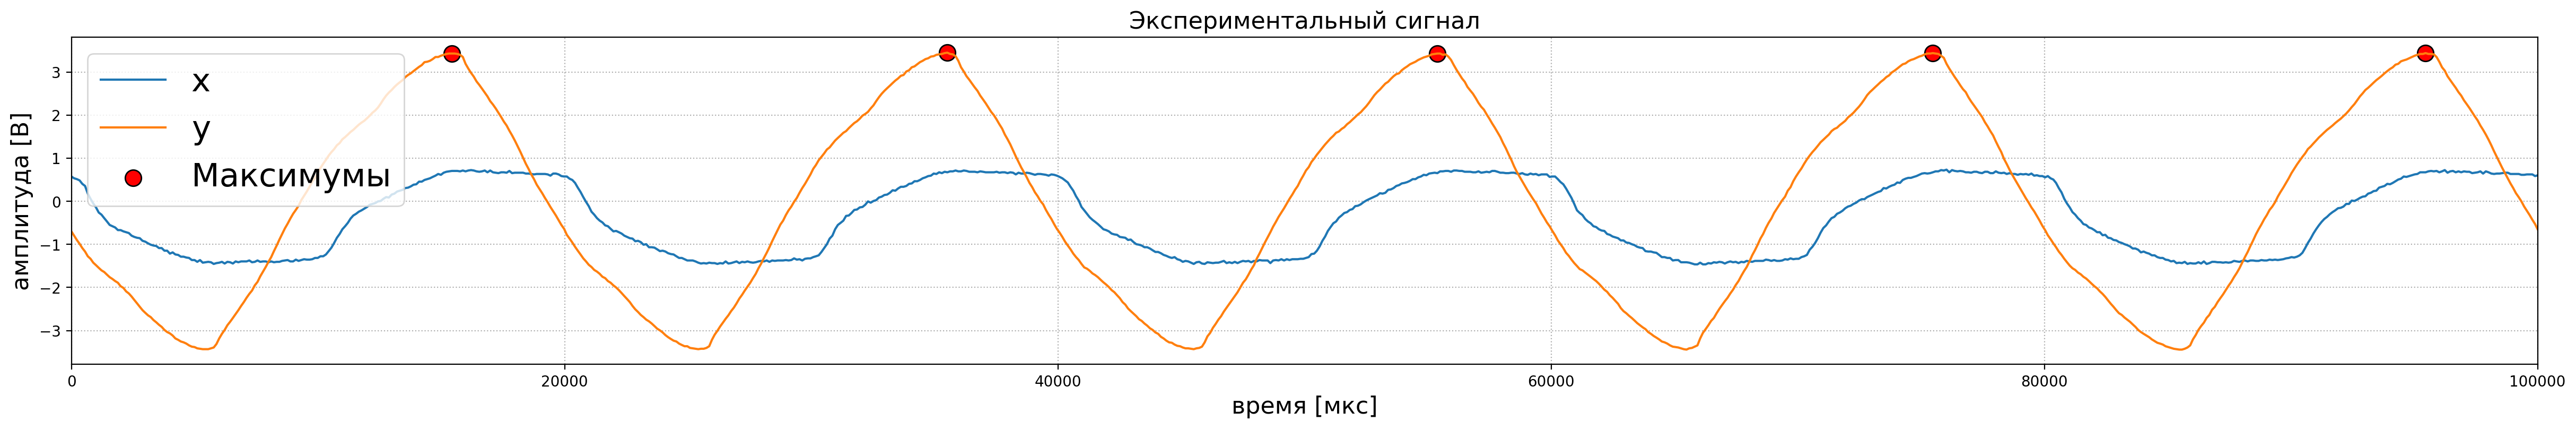
\includegraphics[width = 1\textwidth]{raw_signals.png}
    \caption{сигналы полученные в ходе эксперимента}
    \label{fig:raw_signals}
\end{figure}

Несложно алгоритмически найти максимумы в экспериментальном сигнале.
Вскоре это позволит нам разделять периоды сигнала.

Для построения петли гистерезиса произведём следующие операции:
\begin{enumerate}
    \item Нормализуем напряжения по осям x и y
        \subitem Вычтем из каждого сигнала его среднее значение(сдвинем математическое ожидание случайных величин x и y в 0)
        \subitem Отнормируем сигналы поделив экспериментальные значения на зарегистрированный максимум 
    \item Переведём ось x из относительных единиц в Эрстеды. Для этого растянем сигнал в $I_{amp} \sqrt{2} \cdot 150$, где $I_{amp}$ - ток через амперметр(7).
    \item Усредним сигналы по трём периодам.
\end{enumerate}

\begin{figure}[htbp]
    \centering
    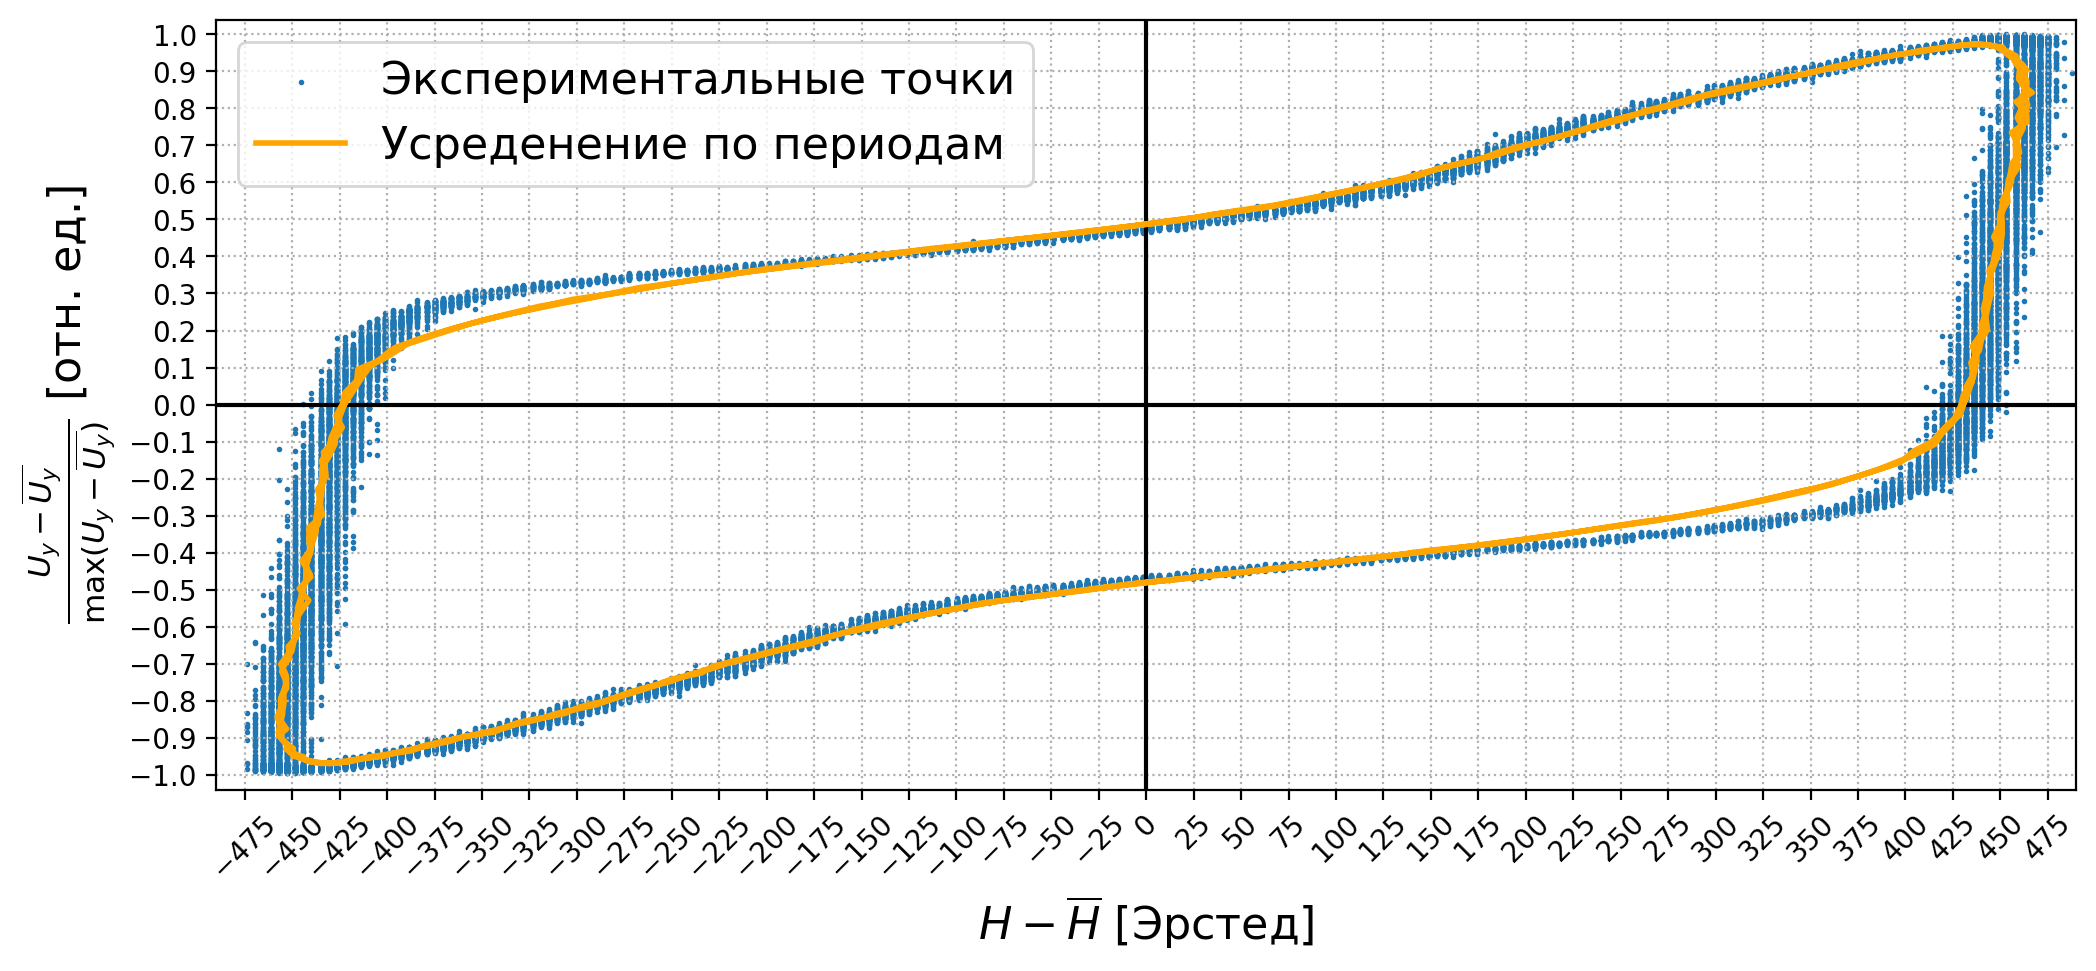
\includegraphics[width = 1 \textwidth]{main.png}
    \caption{Петля гистерезиса}
    \label{fig:main}
\end{figure}
По полученному графику несложно определить величину коэрцетивной силы. Для этого построим гистограмму
значений поля $H$ при котором $y$ практически равен нулю(смотрите рисунок \ref{fig:hist_coerr}).

\begin{figure}[htbp]
    \centering
    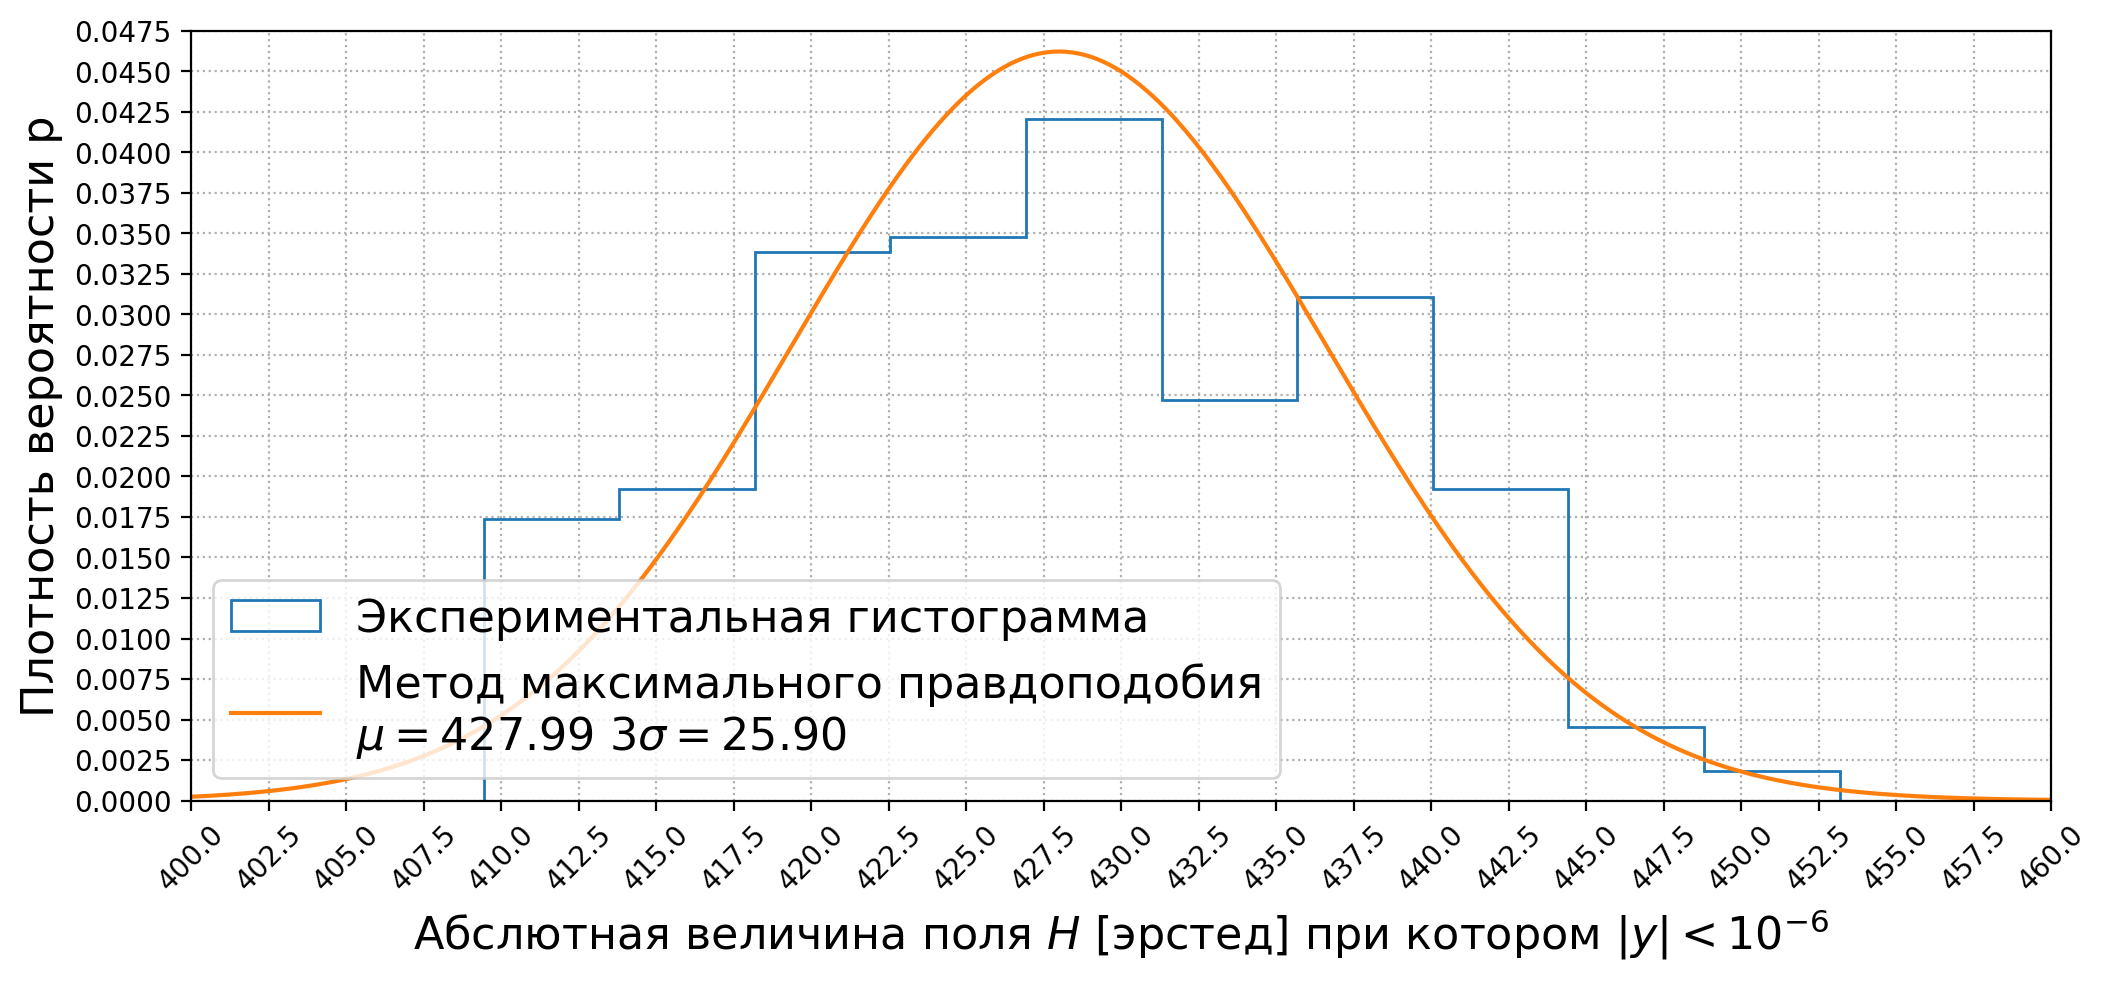
\includegraphics[width = 0.9 \textwidth]{hist_coerr.png}
    \caption{Распределение абсолютной величины коэрцетивной силы}
    \label{fig:hist_coerr}
\end{figure}

Таким образом, величина коэрцетивной силы оказалась равной 
\textcolor{defenition}{$H_{c} = 430 \pm 30$ Эрстед}.

Аналогично можно определить величину поля насыщения. Для этого найдём среднее значения 
полей при которых $||y| - 1| < 10^{-3}|$, а для оценки случайной ошибки посчтиаем три стандартных отклонения.
В результате получим \textcolor{defenition}{$H_{\text{s}} = 460 \pm 20$ Эрстед}.

Приведённые выше результаты учитывают только случайную ошибку. 
Аппаратная ошибка складвается из ошибки оперделения величины тока(возьмём одно деление амперметра $\sim 1\%$)
и из дискретности значений АЦП. Диапазон входных значений АЦП - (-5В, 5В), разрядность - 10 бит. 
А значит ошибка определения напряжения $10 / 2^{10} \sim 10 мВ \sim 0.1 \%$.

Таким образом итоговые значения полей:
\begin{equation}
    H_{s} = 460 \pm 25 \text{ Эрстед} \ \ \ 
    H_{c} = 430 \pm 35 \text{ Эрстед}
\end{equation}

\section*{\textcolor{header}{Вывод}}

В ходе эксперимента удалось определить основные величины гистерезиса. Итоговая
ошибка оказалась равной $\sim 6\%$. При этом основной вклад в ошибку вносит случайная ошибка.

Для улучшения точности вычисляемых значений следует минизировать случайную ошибку. Для этого
следует убрать возможные колебания стола, на котором расположена оптическая система.



\end{document}
